%!TEX root = /Users/rafaeldurelli/Dropbox/Artigos Elaborados/KDM propagation_2015/sbes_2015_kdm_propagation/sbes2015_kdm_propagation.tex

\section{Background} % (fold)
\label{sec:background}

In this section we provide a brief background to Architecture-Driven Modernization (ADM) and Knowledge Discovery Metamodel (KDM). Further, we describe in detail why change propagation in KDM is a complex process.

\subsection{ADM and KDM}

The growing interest in using Model-Driven Development (MDD) to manage software evolution is mainly focused on the reengineering or modernization of legacy systems. Several software migration projects have been carried out with model-driven approaches~\cite{Heckel2008, Andrade:2005, Reus:2006}. %In addition, the 

This growing interest motived OMG to define the ADM initiative~\cite{1686216} which advocates carrying out the reengineering process considering MDD principles. 
ADM is the concept of modernizing existing systems with a focus on all aspects of the current systems architecture and the ability to transform current architectures to target architectures by using all principles of MDD~\cite[p.~60]{Ulrich:2010:IST:1841736}. 


Figure~\ref{fig:ADM_shorseshoe} depicts the horseshoe model (i.e., horseshoe is basically a left-hand
side, a right-hand side and a bridge between the sides) which was adapted to ADM. %Please note that it contains all the traditional phases and some MDD's keywords, such as PSM and  PIM. The traditional phases adapted to ADM are:

\begin{itemize}

\item \textbf{Reverse Engineering}: herein a reverse engineering is realized, it takes a legacy system to be modernized as input, then the knowledge is extracted and a PSM is generated. In addition the PSM serves as the basis for the generation of a PIM, which is called KDM (see Section~\ref{sec:KDM});

\item \textbf{Restructuring}: in this phase a set of restructuring/refactoring can be applied into a KDM's instance by means of M2M transformations;

\item \textbf{Forward Engineering}: then a forward engineering is carried out and the source code of the modernized target system is generated.

\end{itemize} 

%Figure~\ref{horseshoe} depicts the ADM modernization domain model where the left side of the horseshoe is the current state of a busines/it architecture ``as is'' and the right side is what we want to get after the modernization ``to-be''. %One common path followed by IT is to focus on the technical architecture. Generally, the cost of this approach is lower and project duration shorter because the data and application architectures remain largely intact but there is almost no impact or value to the business. 

%On the other hand, a modernization which seeks to provide value to the business, would need to change the application and data architecture, which in turn would rely on an analysis of requirements stemming from shifts to the business architecture. These types of projects are of a longer duration, require more investment, and deliver significantly more value to the business.


\begin{figure}[!ht]
\centering
  % Requires \usepackage{graphicx}
 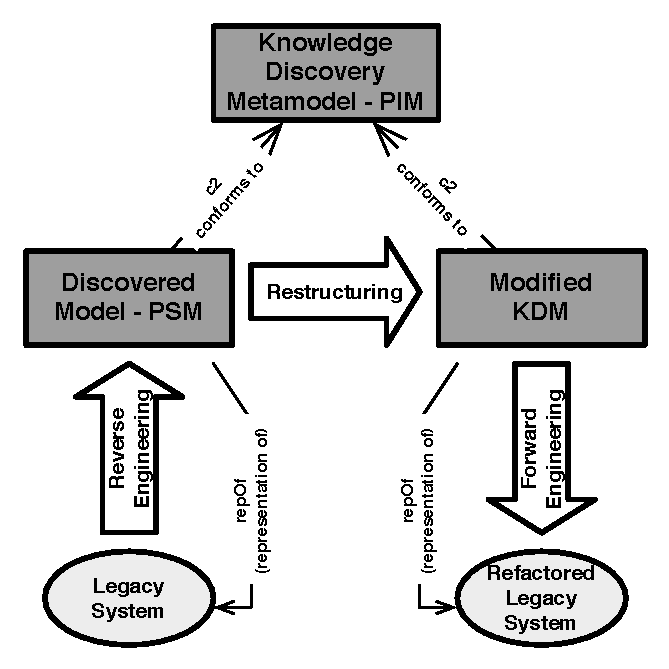
\includegraphics[scale=0.55]{figuras/horseshoes}
\caption{Horseshoe Modernization Model. This figure is adapted from~\cite{OMG_ADM}.}
\label{fig:ADM_shorseshoe}
\end{figure}

In order to perform a systematic modernization as depicted in Figure~\ref{fig:ADM_shorseshoe}, ADM introduces several modernization standards, among them there is the Knowledge Discovery Metamodel (KDM).
%However, herein we focus on KDM because it is the key cornerstone of ADM and the main ideas of our research. 
KDM is an OMG specification adopted as ISO/IEC 19506 by the International Standards Organization for representing information related to existing software systems. 
The goal of the KDM standard is to define a metamodel to represent all the different legacy software artifacts involved in a legacy information system (e.g. source code, user interfaces, databases, business rules, etc.). %The metamodel of the KDM standard provides a comprehensive high-level view of the behavior, structure and data of legacy information systems by means of a set of facts. 
Please, not that although KDM is a metamodel, its main purpose is not the representation of models related strictly to the source code nature such as Unified Modeling Language (UML). While UML can be used to generate new code in a top-down manner, an ADM-based process using KDM starts from the different legacy software artifacts and builds higher-abstraction level models in a bottom-up manner through reverse engineering techniques. %KDM can be seen from different perspectives, as follows: (\textit{i}) KDM can be considered as a metamodel to represent legacy knowledge models, (\textit{ii}) most of the KDM specification is a definition of a language- and platform-independent ontology of legacy information systems and (\textit{iii}) KDM is a common interchange format that makes the interoperability between the reverse engineering tools and modernization tools possible.

KDM specification owns some KDM domain, each domain defines an architectural viewpoint. In order to define the catalogue of refactoring for the KDM we need to focus just on the Program Element Layer - more specifically  in the Code Package, which represents the code elements of a program (classes, fields and methods) and their associations. %We are interested in the Code Package once our catalogue is based on fine-grained refactorings, i.e., refactorings to be applied into classes, fields and methods. 
Therefore, it is important to dig a little deeper in the Code Package.
%
%In a given KDM instance, each instance of the code meta-model element represents some programming language construct, determined by the programming language of the existing software system. Each instance of a code meta-model element corresponds to a certain region of the source code in one of the artifacts of the existing software system. In addition, 
%
The Code Package consists of $24$ classes and contains all the abstract elements for modeling the static structure of the source code. In Table~\ref{tab:mappingCodeToKDM} is depicted some of them. This table identifies KDM metaclasses possessing similar characteristics to the static structure of the source code. Some metaclasses can be direct mapped, such as Class from object-oriented language, which can be easily mapped to the ClassUnit metaclass from KDM.


\begin{table}[!h]
\caption{Metaclasses for modeling the static structure of the source-code}
\label{tab:mappingCodeToKDM}
\centering
\begin{tabular}{|>{\centering}p{3cm}|>{\centering}p{3cm}|}
\hline 
Source-Code Element & KDM Element\tabularnewline
\hline 
\hline 
Class & ClassUnit\tabularnewline
\hline 
Interface & InterfaceUnit\tabularnewline
\hline 
Method & MethodUnit\tabularnewline
\hline 
Field & StorableUnit\tabularnewline
\hline 
Local Variable & Member\tabularnewline
\hline 
Parameter & ParameterUnit\tabularnewline
\hline 
Association & KDM RelationShip\tabularnewline
\hline 
\end{tabular}
\end{table}

  %\begin{figure}[!ht]
  %\centering
  % Requires \usepackage{graphicx}
    %\includegraphics[scale=0.39]{FIGURAS_DA_REFATORACAO/ProgramLaye0r}
  %\caption{Chunk of the Code Package (OMG Group~\cite{OMGADM})}
  %\label{fig:programLayer}
  %\end{figure}

 %As can be seen in Figure~\ref{fig:programLayer} the root metaclass is \textit{ComputationalObject} which has two sub-metaclasses, i.e., \textit{DataElement} and \textit{ControlElement}. The former sub-metaclass, \textit{DataElement}, is a generic modeling element that defines the common properties of several concrete classes that represent the named data items of existing software systems, for example, global and local variables, record files, and formal parameters. \textit{DataElement} has five sub-metaclasses - \textit{StorableUnit}, \textit{IndexUnit}, \textit{ItemUnit}, \textit{ParameterUnit} and \textit{MemberUnit}. \textit{StorableUnit} is a concrete  sub-metaclass of the \textit{StorableElement} meta-class that represents variables of the existing software system. \textit{IndexUnit} class is a concrete subclass of the \textit{DataElement} class that represents an index of an array datatype. Instances of \textit{ItemUnit} class are endpoints of KDM data relations which describes access to complex datatypes. \textit{ParameterUnit} class is a concrete subclass of the \textit{DataElement} class that represents a formal parameter; for example, a formal parameter of a procedure. \textit{MemberUnit} class is a concrete subclass of the \textit{DataElement} class that represents a member of a class type. Finally, the latter, \textit{ControlElement} is a sub-metaclass that contains two sub-metaclasses - \textit{MethodUnit} and \textit{CallableUnit}. \textit{MethodUnit} element represents member functions owned by a \textit{ClassUnit}, including user-defined operators, constructors and destructors. The \textit{CallableUnit} represents a basic stand-alone element that can be called, such as a procedure or a function. %As can be seen below the dashed line in Figure~\ref{fig:programLayer} there are also the following enumerations: ``\textit{ExportKind}'', ``\textit{StorableKind}'', ``\textit{CallableKind}'', ``\textit{MethodKind}'', which are sets os literals used as properties of the metaclasses.
 


\begin{figure}
	\centering
	% Requires \usepackage{graphicx}
	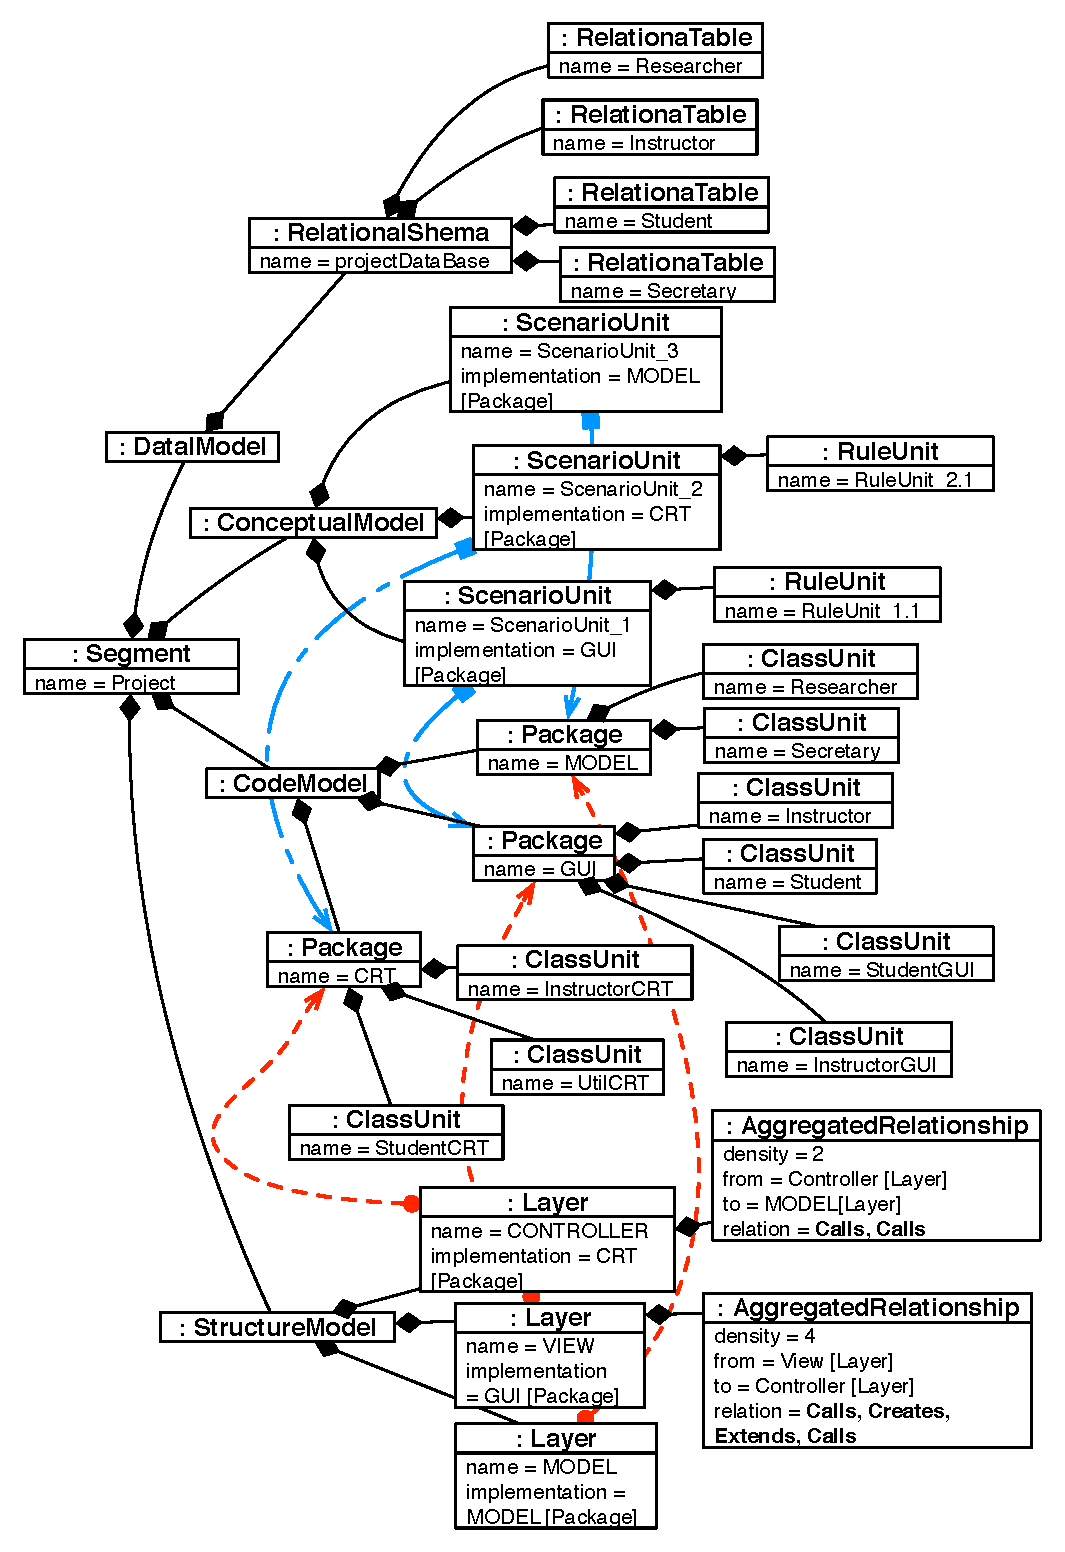
\includegraphics[scale=0.53]{figuras/TreeNewJoint}
	\caption{A bird's eye view of a KDM's instance.}
	\label{fig:allKDMLayers}
\end{figure}

\subsection{Change Propagation in KDM} % (fold)
\label{sub:change_propagation_in_kdm}

In our previous work~\cite{IRIDurelliCatalogo}, we introduced a refactoring catalogue for KDM for managing evolution of a software system. This paper served as a starting point to investigate how the changes affect the KDM's levels. For instance, depending on the refactoring a set of metaclasses must to be create, updated and even removed, these operations may cause minor or major changes to be propagated into other KDM's metaclasses. In order to explain the propagation of changes in KDM consider the Figure~\ref{fig:allKDMLayers}. This figure depicts the corresponding, though simplified KDM instance of system depicts in Figure~\ref{fig:system}. It illustrates a KDM instance as a UML object diagram for the sake of simplicity. Notice that due space limitations some elements are not depicted in this figure.

As we can see, a KDM's instance can be understood as a tree where we have a specially node called the root of the tree. Then the remaining nodes are partitioned into $\textit{M} >= 0$ joint sets $T_{1}, T_{2}, ..., T_{n}$, and each of these sets is a subtree.  Each nodes represent a metaclass that make up the system depicted in Figure~\ref{fig:system}. The edges represent the relationship between the metaclasses.


%each KDM's levels/packages can be partitioned both horizontally and vertically; in both cases its metaclasses are closely related and interconnected. %The relations form the key concept of modernization by means of KDM, since they invoke the needs for change propagation. 
%
The root is the metaclass \texttt{Segment}. There are four subtrees rooted at \texttt{StructureModel}, \texttt{CodeModel}, \texttt{ConceptualModel}, and \texttt{DataModel}, respectively. 
The tree rooted at \texttt{StructureModel} has three \texttt{Layers}, \texttt{CONTROLLER}, \texttt{VIEW}, and \texttt{MODEL} - they are connected by the metaclasses \texttt{AggregatedRelationship} (see Figure~\ref{fig:system} and Figure~\ref{fig:allKDMLayers}).

The tree rooted at \texttt{CodeModel} has three instance of the metaclass \texttt{Package} - \texttt{CRT}, \texttt{GUI}, and \texttt{MODEL}, respectively. Further, each package contains a set of classes, for instance, the package \texttt{MODEL} has two instance of the metaclass \texttt{ClassUnit}, \texttt{Researcher}, and \texttt{Secretary}, respectively.

The tree rooted at \texttt{ConceptualModel} also has three subtree - herein represented by the metaclass \texttt{ScenarioUnit}. Further, each node of a tree is the root of a \texttt{RuleUnit}. Finally, the \texttt{DataModel} has one subtree - \texttt{RelationalSchema}, which represent the system's data base schema. It contains four subtree - \texttt{Secretary}, \texttt{Researcher}, \texttt{Instructor}, and \texttt{Student}, where each node is an instance of the metaclass \texttt{RelationalTable}. 


%If we consider the horizontal partitioning, we can identify four branches. Each branches represents a KDM's levels/packages just as in the Figure~\ref{fig:system}. The lower branch, \texttt{StructureModel}

% However, in this Figure, each KDM's levels/packages are grouped by its root elements. For instance, the node labeled \texttt{StructureModel} is the root metaclass for all architecture elements.  


%on the lower level it is possible to see the metaclasse \texttt{StrutureModel} that is the root metaclasses of all architecture elements. As can be seen it contains three Layers where each bounded dashed lines shape represents a KDM's levels/package.



% . Each package is used to represent an specific artifact, such as, source-code, structure elements, databases, and conceptual elements. As stated in Section~\ref{sec:background} KDM is organized into four layers. In Figure~\ref{fig:allKDMLayers} three of them is shown. The squiggle (leftmost) part represents the Abstract Layer, which defines a set of meta-model elements that represent domain-specific and application-specific abstractions. The stipple (middle) part represents the Resource Layer, which describes common patterns for representing the operating environment of existing software systems. Finally, the highlighted in grey (rightmost) defines a large set of meta-model elements whose purpose is to provide a language-independent intermediate representation for various constructs determined by common programming languages.
 

%Further, if we consider the horizontal partitioning, we can identify four levels, each representing a different view of an system instantiated in KDM. The lowest level represents all the physical artifacts owned in a system. Its parent level, called KDM's metaclasses, represents the particular KDM's metaclasses, which conforms to an specific artifact. The level above represents the system specification. Finally, the highest level represent all the KDM's models, each model defines a set of metaclasses to represent the physical and logical elements of software as well as their relationships at various levels of abstraction.

%In order to cope with propagation of the refactoring changes across any KDM's subtree dependent abstraction levels, keeping all models synchronized

In the context of model-driven refactoring, if any change occurs at any KDM's subtree the change should be propagated to other elements.
%
%These levels indicate problems related to KDM propagation of changes. 
%
For instance, when the elements of \texttt{CodeModel} suffer any kind of changes (e.g., are refactored), its instances, i.e., \texttt{ClassUnits}, \texttt{MethodUnits}, \texttt{StorableUnits}, etc, and related elements must be adapted accordingly so that their validity and correctness is preserved respectively. In addition, if we want to preserve others parts of KDM, like the system's structure and the business rules the  \texttt{StructureModel} and \texttt{ConceptualModel} also need to adapt, respectively. %What is more, as we have mentioned, in practice there are usually at least one instance of each KDM's model applied in a single system, e.g., the system architecture conforms to Structure Model, the source-code conforms to Code Model, etc. 
In general, a change at one KDM's model should trigger a cascade of changes at other models. We call such sequences of adaptations change propagation.

As we can see in Figure~\ref{fig:allKDMLayers}, there are not only horizontally relations between the models, but the elements of the system can also be vertical related across the vertical partitions. A few examples are denoted by the red/blue dashed arrows. For instance, there is a relation between a \texttt{CodeModel} (its respective metaclasses) with the \texttt{StructureModel} - which means that a change in one of the ends of the relation can influences the other.

Considering these KDM's models leads to evolution of each affected model separately. However, this is a highly time- consuming and error-prone solution since we need a domain expert who is able to identify all the affected models and propagate the changes. Following we present our approach to detect and propagate all the changes throughout all KDM's levels.

